\documentclass[11pt,a4paper]{article}
\usepackage[utf8]{inputenc}
\usepackage[T1]{fontenc}
\usepackage[spanish,es-noshorthands]{babel}
\usepackage{amsmath,amssymb,amsthm}
\usepackage{bm}
\usepackage{geometry}
\geometry{margin=2.5cm}
\usepackage{graphicx}
\graphicspath{{../figuras/}}
\usepackage{float}
\usepackage{xcolor}
\usepackage{hyperref}
\hypersetup{colorlinks=true,linkcolor=blue!50!black,citecolor=blue!50!black,urlcolor=blue!50!black}
\usepackage{enumitem}
\usepackage{booktabs}
\newtheorem{definition}{Definición}
\newtheorem{remark}{Observación}
\newcommand{\R}{\mathbb{R}}
\newcommand{\thetavec}{\bm{\theta}}
\newcommand{\transp}{^{\top}}
\newcommand{\promptIA}[1]{\begin{center}\fcolorbox{gray}{gray!8}{\parbox{0.9\linewidth}{\small\textbf{[FIGURA -- PROMPT IA]}\\[2pt]#1}}\end{center}}
\title{\textbf{R3 --- Conclusiones, novedad y trabajo futuro}\\[2pt]\large Qué logramos, qué es aporte propio y qué queda abierto}
\author{Proyecto Wilson--Cowan --- Iniciación a la I+D ITBA}
\date{\today}
\begin{document}
\maketitle
\tableofcontents
\bigskip

%========================================================
\section{Síntesis del proyecto en una página}
%========================================================

Este documento cierra el paquete: recoge lo que se hizo, separa lo prestado de lo
propio y ordena lo que queda pendiente. Para los números y las figuras de fondo,
remitimos a \textbf{R1} (resultados de identificación sintética) y a \textbf{R2}
(datos reales); para el andamiaje conceptual, a \textbf{M5} (identificabilidad:
Fisher + SVD), \textbf{M6} (diseño de estímulo / OED) y \textbf{B5} (control en
lazo cerrado).

El proyecto se resume en cuatro verbos encadenados sobre el modelo de
Wilson--Cowan (WC)~\cite{wc1972}:

\begin{description}[leftmargin=1.4em,style=nextline]
  \item[Identificar.] Recuperar los \textbf{10 parámetros} de WC
  ($w_{EE},w_{EI},w_{IE},w_{II},\tau_e,\tau_i,a_e,a_i,\theta_e,\theta_i$) a partir
  de trayectorias sintéticas con ruido, usando una \emph{Neural ODE} como
  identificador \emph{gray-box}~\cite{chen2018,rackauckas2020}. El arranque es
  ``ignorante'': no se le da a la red el valor verdadero de ningún parámetro. No
  identificamos solo los 4 pesos de conexión, sino los 10 escalares.

  \item[Diagnosticar.] Antes de confiar en los estimados, preguntar
  \emph{cuáles son recuperables}. La matriz de información de Fisher (FIM) y su
  descomposición en valores singulares (SVD) responden esto sin siquiera
  entrenar: la dirección singular más débil apunta casi por completo a
  $\bm{w_{II}}$ (autoinhibición). Es el \textbf{cuello de botella}: predicho por la
  geometría de la FIM y \emph{confirmado} después por el barrido de ruido (error
  $\approx 41\%$ a $\sigma=0{,}10$). Ver R1 y M5.

  \item[Mitigar.] Tres palancas, todas con método publicado detrás:
  \emph{subset selection} (fijar el parámetro plano en su prior),
  \emph{regularización} (penalizar la dirección débil en vez de fijarla) y
  \emph{diseño de estímulo} (OED: elegir qué inyectar para que la FIM ``vea''
  mejor a $w_{II}$). Ver R1 y M6.

  \item[Validar orientado al control.] El desenlace: el modelo identificado
  alimenta un controlador IMC en lazo cerrado y se mide, \emph{end-to-end}, si la
  fragilidad de $w_{II}$ contamina el seguimiento. \textbf{No lo hace}: la acción
  integral del IMC absorbe el error aun con $w_{II}$ mal recuperado. Ver B5.
\end{description}

La moraleja del proyecto en una frase: \emph{la identificabilidad de WC es
estructural (hay una dirección intrínsecamente plana, $w_{II}$), pero esa
fragilidad se queda en la identificación y no se propaga al objetivo final, que es
controlar el régimen theta--gamma con estímulos realizables por optogenética.}

%========================================================
\section{Novedad: encuadre honesto}
%========================================================

La regla que seguimos para no inflar la contribución es una plantilla explícita:

\begin{center}
\fcolorbox{gray}{gray!8}{\parbox{0.9\linewidth}{\centering
\emph{``Usa métodos de \textbf{X} (de tal referencia) aplicados a \textbf{Y}
con \textbf{Z} (el cambio/hallazgo propio)''.}}}
\end{center}

Es decir: los \textbf{métodos son prestados y citados}; el \textbf{aporte} es la
\emph{combinación} de todos ellos sobre un mismo modelo, más el \emph{hallazgo}
concreto ($w_{II}$) y la observación de que la \emph{fragilidad no llega al
control}. Desglosado por eje:

\begin{itemize}[leftmargin=1.4em]
  \item \textbf{Identificabilidad.} Métodos de \emph{Fisher + SVD},
  \emph{subset selection} y \emph{profile likelihood} --- Golub \& Van
  Loan~\cite{golub2013} (la maquinaria SVD/QR), Chu \& Hahn~\cite{chuhahn2007}
  (selección de subconjunto de parámetros sobre la matriz de sensibilidad) y
  Raue et al.~\cite{raue2009} (profile likelihood, el estándar de
  identificabilidad práctica) --- \emph{aplicados a} WC identificado con Neural
  ODE, \emph{con} el hallazgo de que $w_{II}$ es el cuello de botella, predicho
  sin entrenar y confirmado bajo ruido.

  \item \textbf{Diseño de estímulo.} Métodos de \emph{OED / excitación
  persistente} --- Ljung~\cite{ljung1999} (identificación de sistemas, entrada
  persistentemente excitante) y Plate et al.~\cite{plate2024} (OED para UDEs con
  Fisher) --- \emph{aplicados a} WC, \emph{con} la ponderación explícita del
  criterio hacia el cuello de botella (la curva en V del OED ponderado, óptimo en
  $\rho=0{,}5$; ver M6 y R1).

  \item \textbf{Modelado.} \emph{Neural ODE gray-box / UDE} ---
  Chen et al.~\cite{chen2018} (Neural ODE) y Rackauckas et
  al.~\cite{rackauckas2020} (universal differential equations) --- \emph{aplicado
  a} los \textbf{10 parámetros} de WC (no solo los 4 pesos), \emph{con} el arranque
  ignorante y la validación orientada al control.
\end{itemize}

\paragraph{Aporte global.} La \textbf{combinación} de estas piezas sobre un mismo
modelo, más el \textbf{hallazgo ($w_{II}$)}, más el resultado de que la
\textbf{fragilidad no se propaga al control}. Formulado con cautela: \emph{hasta
donde vimos, es el primer trabajo que identifica los 10 parámetros de
Wilson--Cowan con una Neural ODE, diagnostica con Fisher+SVD qué se recupera
($w_{II}$ el límite) y demuestra que esa fragilidad no llega al control en lazo
cerrado.}

\paragraph{El antecedente más cercano a diferenciar.} \emph{Adaptive Stimulus
Design for Dynamic Recurrent Neural Network Models} (PMC6349832) ya muestra que
estímulos diseñados óptimamente recuperan mejor las constantes de tiempo y los
pesos de conexión de un modelo neuronal. \textbf{No nos invalida}, pero hay que
nombrarlo con honestidad: (i) el modelo es un RNN dinámico, \emph{no} Wilson--Cowan;
(ii) \emph{no cierra el lazo de control}. Nuestro diferencial es precisamente el
modelo WC específico y la validación \emph{end-to-end} sobre el controlador.

\begin{remark}
Toda afirmación de novedad descansa en una búsqueda acotada (pocas queries, sin
bases pagas). Para afirmarla en serio hace falta una búsqueda sistemática
(Scholar + arXiv + IEEE Xplore) y, sobre todo, contrastar con el tutor, que
conoce su línea mejor que cualquier búsqueda automática.
\end{remark}

%========================================================
\section{Qué se puede afirmar vs.\ qué queda abierto}
%========================================================

La honestidad científica exige separar la conclusión firme del \emph{caveat}.

\paragraph{Se puede afirmar (evidencia dentro del setup).}
\begin{itemize}[leftmargin=1.4em]
  \item Con datos sintéticos limpios y multiple shooting, los 10 parámetros de WC
  se identifican bien desde arranque ignorante (ver R1, ajuste sobre trayectoria
  de test tipo chirp).
  \item $w_{II}$ es la dirección estructuralmente débil: la SVD de la FIM lo
  predice \emph{sin entrenar} y el barrido de ruido lo confirma como el peor
  parámetro. Es una predicción que se cumple, no una observación aislada.
  \item El error de identificación de $w_{II}$ \textbf{no se propaga} al
  seguimiento en lazo cerrado dentro del régimen y del controlador IMC probados
  (ver B5).
\end{itemize}

\paragraph{Queda abierto (caveats explícitos).}
\begin{itemize}[leftmargin=1.4em]
  \item \textbf{Semillas redundantes en el OED ponderado.} La corrida del OED
  ponderado usó pocas semillas (5\,$\rho$ $\times$ 3 seeds); parte de la variación
  entre semillas es redundante y no permite poner barras de error confiables sobre
  el óptimo $\rho=0{,}5$. La forma en V es sugerente, no concluyente.
  \item \textbf{Familia de estímulo y paso $dt$ no concluyentes.} El barrido por
  familia con $dt$ grande ($\approx0{,}2$) mezcla el efecto de la familia con el
  del error de integración; con $dt$ grueso no se puede separar limpiamente qué
  estímulo ayuda más ni cuánto pesa el discretizado (ver R1, familia + límite de
  $dt$).
  \item \textbf{Datos reales con input débil.} En datos que no son WC puro, la
  señal de entrada es débil y el modelo de observación (LFP) no está cerrado; los
  resultados de R2 son exploratorios, no una identificación validada.
\end{itemize}

%========================================================
\section{Conclusiones por eje}
%========================================================

\paragraph{Modelo / simulador.} El simulador de WC (forma canónica con offsets
$k_e,k_i$ derivados para que el reposo sea equilibrio; salida $y=E-I$) es sólido y
reproduce el ciclo límite objetivo. Sirve tanto de generador de datos sintéticos
como de planta para el control. Es la base común de todo el paquete.

\paragraph{Identificación sintética.} La Neural ODE gray-box identifica los 10
parámetros desde arranque ignorante con datos limpios. El pipeline (multiple
shooting, reparametrización softplus para positividad, integrador RK4
diferenciable) funciona y converge. Es la prueba de concepto que habilita todo lo
demás.

\paragraph{Identificabilidad.} El resultado conceptual más limpio del proyecto:
existe una dirección plana estructural en el espacio de parámetros, dominada por
$w_{II}$. La Figura~\ref{fig:valle} lo ilustra: la FIM tiene un valle casi plano a
lo largo del cual el costo apenas cambia, y ese valle se alinea con $w_{II}$. Se
predijo con Fisher+SVD y se confirmó con ruido. Las palancas de mitigación (fijar,
regularizar, rediseñar el estímulo) atacan exactamente esa dirección.

\begin{figure}[H]
  \centering
  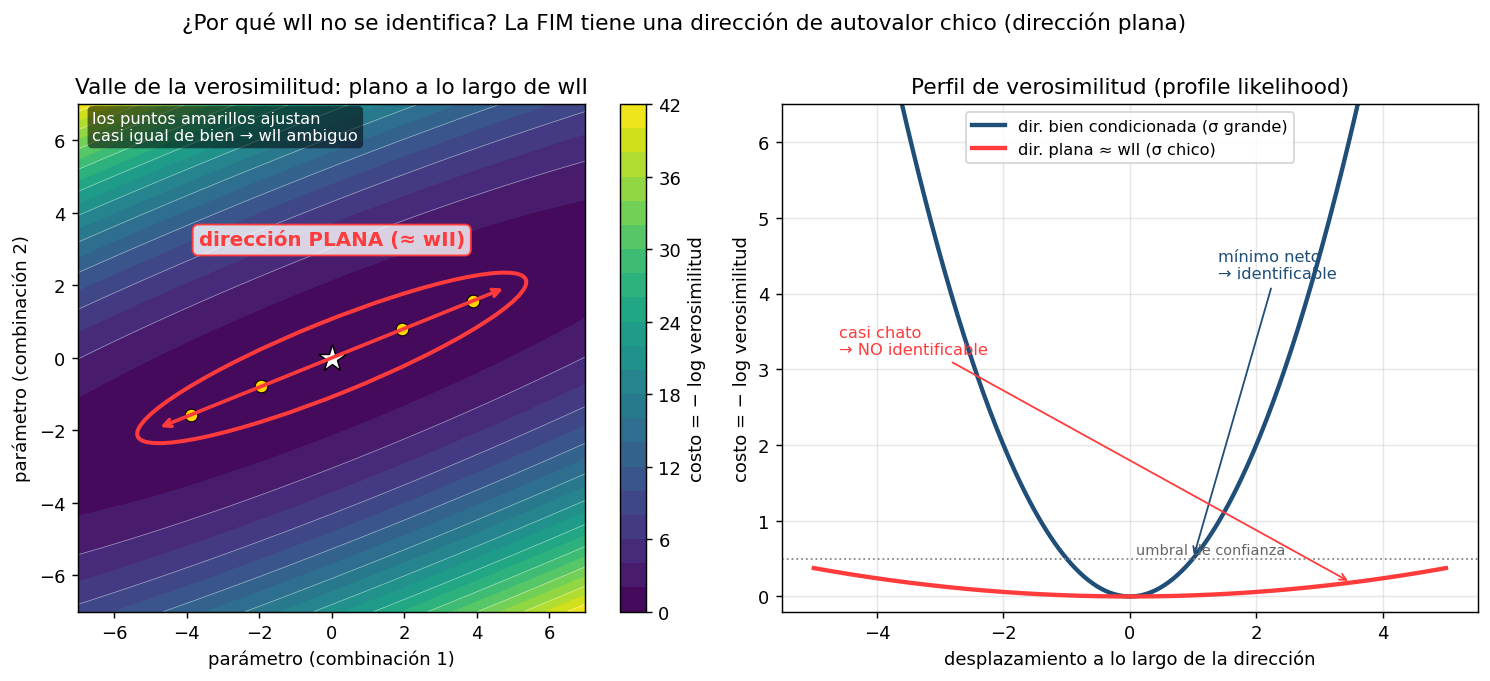
\includegraphics[width=0.75\linewidth]{valle_plano_svd_fim.png}
  \caption{El ``valle plano'' de la FIM: a lo largo de la dirección singular más
  débil el costo casi no cambia, y esa dirección apunta a $w_{II}$. Por eso $w_{II}$
  es el parámetro difícil de identificar. (figura del proyecto)}
  \label{fig:valle}
\end{figure}

\paragraph{Control.} El desenlace que da sentido al proyecto: la fragilidad de la
identificación \textbf{no se propaga}. La Figura~\ref{fig:control} compara el
seguimiento en lazo cerrado usando los parámetros estimados $\hat{\thetavec}$
frente a los verdaderos; las trayectorias son prácticamente indistinguibles. La
acción integral del IMC compensa el error de modelo, incluso con $w_{II}$ mal
recuperado. La identificabilidad imperfecta no es un impedimento para el objetivo
de control.

\begin{figure}[H]
  \centering
  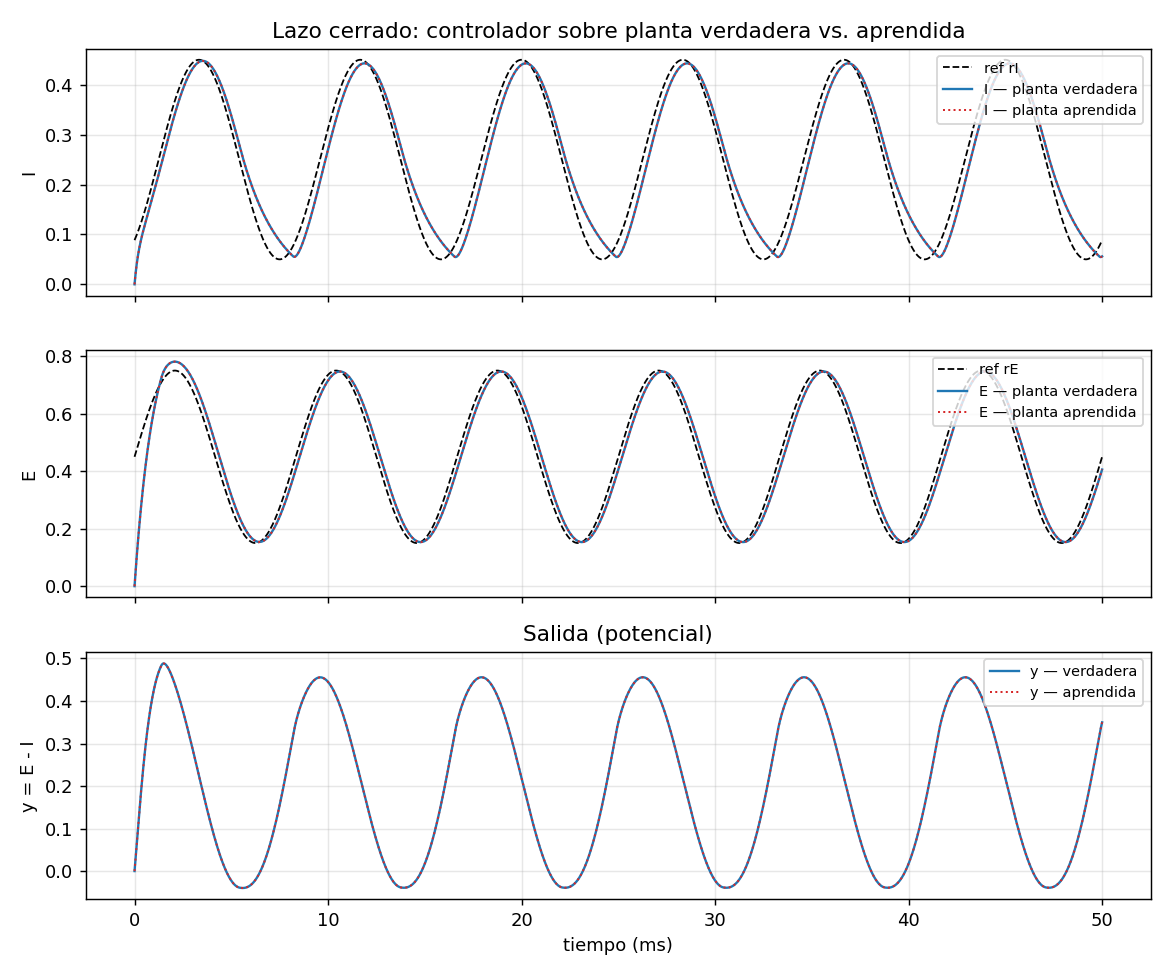
\includegraphics[width=0.75\linewidth]{closed_loop_compare.png}
  \caption{Control en lazo cerrado: seguimiento con los parámetros estimados
  $\hat{\thetavec}$ vs.\ los reales. La fragilidad de identificar $w_{II}$ no
  contamina el seguimiento. (figura del proyecto)}
  \label{fig:control}
\end{figure}

\paragraph{Datos reales.} Es el frente menos maduro. Con datos que no son WC puro,
el input es débil y falta un modelo de observación (LFP) cerrado. Lo de R2 es una
exploración honesta, no una identificación validada; deja el camino marcado para el
trabajo futuro.

%========================================================
\section{Trabajo futuro}
%========================================================

Cinco direcciones, ordenadas de más concreta a más ambiciosa:

\begin{enumerate}[leftmargin=1.6em]
  \item \textbf{OED ponderado realizable.} Repetir la curva en V con estímulos
  \emph{conmutados} (on/off, $\ge 0$), como los que permite la
  optogenética, con $dt$ fino (para separar el efecto del estímulo del error de
  integración) y varias realizaciones de ruido para poner \textbf{barras de
  error} sobre el óptimo $\rho=0{,}5$. Cierra el caveat de las semillas
  redundantes.

  \item \textbf{Gray-box real + modelo de observación LFP.} Activar el término de
  corrección aprendible (\texttt{use\_correction=True}) para capturar dinámica que
  WC puro no modela, y agregar un modelo de observación (LFP) que conecte el estado
  $(E,I)$ con la señal medida. Es el paso necesario para datos que no son WC puro.

  \item \textbf{Cerrar PINN vs.\ Neural ODE bajo ruido.} Completar la comparación
  entre PINN y Neural ODE en el régimen de ruido, lo que requiere extender la PINN
  a los 10 parámetros (hoy está en los 4 pesos). Resuelve una comparación que quedó
  a medias.

  \item \textbf{Reencuadrar los datos reales como predicción a $k$ pasos.} En vez
  de exigir identificación de parámetros con input débil, plantear el problema como
  predicción a $k$ pasos, y luego calcular FIM/SVD sobre el óptimo real
  encontrado, para diagnosticar qué es identificable \emph{en esos datos concretos}
  antes de forzar valores.
\end{enumerate}

\noindent Estas direcciones alimentan el plan de trabajo del proyecto y refuerzan
la contribución sin cambiar el encuadre honesto: seguir usando métodos prestados y
citados, y sumar valor en la aplicación, el hallazgo y la validación.

%========================================================
\begin{thebibliography}{9}

\bibitem{wc1972} H. R. Wilson y J. D. Cowan, ``Excitatory and inhibitory
interactions in localized populations of model neurons'', \emph{Biophysical
Journal} 12(1):1--24, 1972.

\bibitem{chen2018} R. T. Q. Chen, Y. Rubanova, J. Bettencourt y D. Duvenaud,
``Neural Ordinary Differential Equations'', \emph{NeurIPS}, 2018.

\bibitem{rackauckas2020} C. Rackauckas et al., ``Universal Differential Equations
for Scientific Machine Learning'', arXiv:2001.04385, 2020.

\bibitem{raue2009} A. Raue et al., ``Structural and practical identifiability
analysis of partially observed dynamical models by exploiting the profile
likelihood'', \emph{Bioinformatics} 25(15):1923--1929, 2009.

\bibitem{chuhahn2007} Y. Chu y J. Hahn, ``Parameter set selection for estimation
of nonlinear dynamic systems'', \emph{AIChE Journal} 53(11):2858--2870, 2007.

\bibitem{ljung1999} L. Ljung, \emph{System Identification: Theory for the User},
2\textsuperscript{a} ed., Prentice Hall, 1999.

\bibitem{plate2024} C. Plate et al., ``Optimal experimental design for universal
differential equations'', 2024.

\bibitem{golub2013} G. H. Golub y C. F. Van Loan, \emph{Matrix Computations},
4\textsuperscript{a} ed., Johns Hopkins University Press, 2013.

\end{thebibliography}

\end{document}
